\documentclass{VUMIFPSkursinis}
\usepackage{algorithmicx}
\usepackage{algorithm}
\usepackage{algpseudocode}
\usepackage{amsfonts}
\usepackage{amsmath}
\usepackage{bm}
\usepackage{caption}
\usepackage{color}
\usepackage{float}
\usepackage{graphicx}
\usepackage{listings}
\usepackage{subfig}
\usepackage{wrapfig}

\usepackage{enumitem}
%PAKEISTA, tarpai tarp sąrašo elementų
\setitemize{noitemsep,topsep=0pt,parsep=0pt,partopsep=0pt}
\setenumerate{noitemsep,topsep=0pt,parsep=0pt,partopsep=0pt}

% Titulinio aprašas
\university{Vilniaus universitetas}
\faculty{Matematikos ir informatikos fakultetas}
\department{Programų sistemų katedra}
\papertype{Kursinis darbas}
\title{Paieškos proceso ir jos rezultatų pateikimo vartotojams panaudojamumas VUL Santaros klinikų puslapyje}
\titleineng{The Usability of the Search Process and Presenting its Results to the User for VUH Santaros klinikos website}
\status{3 kurso 3 grupės studentas}
\author{Tomas Kiziela}
% \secondauthor{Vardonis Pavardonis}   % Pridėti antrą autorių
\supervisor{doc. Kristina Lapin}
\date{Vilnius – \the\year}

% Nustatymai
% \setmainfont{Palemonas}   % Pakeisti teksto šriftą į Palemonas (turi būti įdiegtas sistemoje)
\bibliography{bibliografija}

\begin{document}
	
% PAKEISTA	
\maketitle
\cleardoublepage\pagenumbering{arabic}
\setcounter{page}{2}

%TURINYS
\tableofcontents

\sectionnonum{Įvadas}
%Įvade apibūdinamas darbo tikslas, temos aktualumas ir siekiami rezultatai.
%Darbo įvadas neturi būti dėstymo santrauka. Įvado apimtis 1–2 puslapiai.
Šiame darbe tiriami informacijos paieškos sprendimai leidžiantys palengvinti Vilniaus universiteto ligoninės (VUL) Santaros klinikų internetinio puslapio santa.lt naudojimą. Tyrime bus atsižvelgta į puslapio navigaciją, informacijos paieškos procesą bei gautų rezultatų pateikimą tradiciniuose ir mobiliuose įrenginiuose.

Kadangi pacientams internetas lengvai prieinamas, darosi įprasta ieškoti informacijos ir registruotis internetu. Tačiau „Trūksta apibendrintos, susistemintos informacijos, kuri pacientui būtų nuolat lengvai prieinama, nes jiems sudėtinga susiorientuoti įstaigų ir interneto svetainių gausoje, rasti ir suprasti skirtingai teikiamą informaciją“\cite{AukšAudInstLt}. VUL Santaros klinikos yra viena didžiausių Lietuvos ligoninių. Joje dirba virš 5000 darbuotojų, o per metus gydoma apie 1 milijonas ambulatorinių (ateinančių iš namų) pacientų\cite{VulSkApieMusLt}. Taigi santa.lt puslapis yra vienas iš pirmųjų internetinių resursų, kurį pasiekia vartotojai. Puslapyje turėtų būti lengva surasti ieškomą informaciją, nes tai padės pacientams priimti sprendimus apie savo sveikatą. Tačiau dabartinė puslapio architektūra turi spragų informacijos paieškos srityje ir naudotojas gali nerasti reikiamos informacijos.

Šio darbo tikslas yra suprojektuoti informacijos architektūrą, kuri leistų pacientams lengviau rasti aktualią informaciją santa.lt puslapyje. Pagrindiniai darbo siekiai yra aiškesnė registracija pas gydytoją ir informacijos apie ligoninės prieinamumą bei struktūrą pasiekiamumas. Galutinis darbo rezultatas - puslapio maketas pabrėžiantis naują informacijos architektūrą.

Uždaviniai:
\begin{enumerate}
	\item Identifikuoti panaudojamumo siekius remiantis literatūros šaltiniais ir internetinių puslapių lankomumo informacija
	\item Išskirti lyginimo kriterijus remiantis literatūros šaltiniais
	\renewcommand*{\theenumii}{\theenumi.\arabic{enumii}}
	\renewcommand{\labelenumii}{\theenumii}
	\begin{enumerate}
		\item Navigacijos
		\item Paieškos
		\item Rezultatų
	\end{enumerate}
	\item Paruošti sprendimo variantus
	\begin{enumerate}
		\item Remiantis panašiais puslapiais ir literatūros šaltiniais išskirti alternatyvius sprendimus
		\item Sukurti sprendimo variantų maketus
		\item Sukurti galutinio sprendimo prototipą
	\end{enumerate}
	\item Išskirti detalius reikalavimus galutinio sprendimo įgyvendinimui
	\item Atlikus literatūros analizę išskirti technologijas padedančias įgyvendinti galutinį sprendimą
\end{enumerate}

\section{Vartotojų poreikių analizė}
Tyrimai nurodo, kad Europoje daugiau nei pusė žmonių bent kartą metuose ieško informacijos apie sveikatą internetu \cite{EuCitizDigHealthEn}. Nagrinėjant santa.lt puslapio srautą randama, kad naudotojai dažniausiai ateina iš (5,5\%) ir yra peradresuojami į (10,4\%) sergu.lt (neįskaitant google.com 19,1\% ir 21,8\% atitinkamai)\cite{AlexaSantaEn}. Taigi galima matyti, kad šie puslapiai turi nemažą vartotojų sutapimą ir būtų naudinga atsižvelgti į tai, kokią įtaką daro vienas kitam. Sergu.lt puslapis skirtas išankstinei visų Lietuvos pacientų registracijai internetu. Tai, kad 1 iš 10 santa.lt vartotojų tiesiogiai pereina į sergu.lt puslapį leidžia tikėti, kad vartotojams yra aktuali registracija pas gydytoją. Santa.lt „Kaip mus rasti?“ skyrelį vartotojai yra aplankę 1,2 milijonus kartų\cite{VulSkKaipMusRastiLt}, 2 kartus daugiau nei skyrelį „Apie mus“\cite{VulSkApieMusLt}, iš to galima daryti prielaidą apie kitą vartotojų siekį - informacijos apie ligoninės klinikų pasiekiamumą.
\vspace{0,5cm}

Atlikus puslapio pažintinę peržvalgą rasti šie panaudojamumo trūkumai:
\begin{enumerate}
	\item Navigacijos
	\renewcommand*{\theenumii}{\theenumi.\arabic{enumii}}
	\renewcommand{\labelenumii}{\theenumii}
	\begin{enumerate}
		\item Pasirinktos kategorijos mažo kontrasto, taigi sunku pastebėti esamą kategoriją
		\item Naviguojant į „Pacientams“, tada „Aktuali informacija“ ir galiausiai „Kaip užsiregistruoti“ pasiekiamas tuščias puslapis
		\item Ant mobilių įrenginių navigacijos juosta beveik neįskaitoma, mygtukai per maži
	\end{enumerate}
	\item Paieškos
	\renewcommand*{\theenumii}{\theenumi.\arabic{enumii}}
	\renewcommand{\labelenumii}{\theenumii}
	\begin{enumerate}
		\item Paieškos laukas turi 20 simbolių limitą, kas neleidžia įvesti ilgesnių paieškos užklausų
		\item Vedant simbolius į paiešką nepasiūlomi užklausos variantai
		\item Nėra filtravimo pagal skirtingas kategorijas
		\item Nėra filtravimo pagal kalbą
		\item Ant mobilių įrenginių sunku paspausti ant paieškos elementų
	\end{enumerate}
	\item Rezultatų
	\renewcommand*{\theenumii}{\theenumi.\arabic{enumii}}
	\renewcommand{\labelenumii}{\theenumii}
	\begin{enumerate}
		\item Rezultatai neturi nuorodos į kategorijas iš kurių jie kilę
		\item Rezultatų lange viskas pateikta teksto pavidalu, nėra grafinių elementų padedančių skirstyti rezultatus pagal kategorijas
		\item Ant mobilių įrenginių prastai matosi rezultato detalės kaip data ir kategorija
	\end{enumerate}
\end{enumerate}
\vspace{0,5cm}
Iš peržvalgos matoma įvairaus sunkumo trūkumų visose kategorijose ir tai, kad puslapis nepritaikytas mobiliems įrenginiams. Tai yra didelė problema, nes mobilieji įrenginiai vis plačiau naudojami \cite{EmergingmHealthEn} ir šių įrenginių vartotojai turėtų galėti laisvai naudotis puslapiu. Galutinis prototipas turi išspręsti šias problemas, neįvedant naujų panaudojomumo trūkumų.
%Medžiagos darbo tema dėstymo skyriuose pateikiamos nagrinėjamos temos detalės:
%pradinė medžiaga, jos analizės ir apdorojimo metodai, sprendimų įgyvendinimas,
%gautų rezultatų apibendrinimas. Šios dalies turinys labai priklauso nuo darbo
%temos. Skyriai gali turėti poskyrius ir smulkesnes sudėtines dalis, kaip
%punktus ir papunkčius.

%Medžiaga turi būti dėstoma aiškiai, pateikiant argumentus. Tekstas dėstomas
%trečiuoju asmeniu, t.y. rašoma ne „aš manau“, bet „autorius mano“, „autoriaus
%nuomone“. Reikėtų vengti informacijos nesuteikiančių frazių, pvz., „...kaip jau
%buvo minėta...“, „...kaip visiems žinoma...“ ir pan., vengti grožinės literatūros
%ar publicistinio stiliaus, gausių metaforų ar panašių meninės išraiškos
%priemonių.
\section{Maketų lyginimo kriterijai}
Panaudojamumo testavimas gali būti atliktas įvairiais metodais. Empiriniai metodai yra plačiausiai naudojami\cite{NielsenUsabilityEn}, tačiau reikalauja daug laiko ir išteklių, todėl pasirinktas vienas iš analitinių metodų. Dėl patirties ir laiko stokos pasirinkta naudoti neformaliausią metodą - euristinį vertinimą.

Maketų palyginimui bus naudojamos laiko patvirtintos Jakob Nielsen euristikos\cite{NielsenHeuristicsEn}. Lentelėje bus išskiriamos 10 euristikų. Kiekvienai euristikai priskiriamas skaičius nuo 0 iki 3 reiškiantis defekto sunkumą, kur 0 - defekto nėra, 1 - smulkus ar kosmetinis defektas, 2 - vidutinio sunkumo defektas, 3 - kritinis defektas. Paskutinis stulpelis nusako, kur ir koks defektas buvo pastebėtas.%\ref{euristikųlentelė}
\begin{center}
\begin{tabular}{ |c|c|c| } 
 \hline
	Euristika & Defekto sunkumas & Komentaras \\ \hline
	1) Būsenos matomumas &  &  \\ \hline
	2) Atitikimas realiam pasauliui  &  &  \\ \hline
	3) Naudotojo valdomas dialogas &  &  \\ \hline
	4) Darna ir standartai &  &  \\ \hline
	5) Klaidų prevencija &  &  \\ \hline
	6) Atpažinimas geriau nei atsiminimas &  &  \\ \hline
	7) Naudojimo lankstumas ir efektyvumas &  &  \\ \hline
	8) Estetiškas ir minimalistinis dizainas &  &  \\ \hline
	9) Remti klaidų atpažinimą, jų priežasčių nustatymą ir taisymą &  &  \\ \hline
	10) Parama ir dokumentacija &  &  \\ \hline
\end{tabular}
\captionof{table}{Euristinis vertinimas}\label{euristikųlentelė}
\end{center}
\subsection{Poskyris}
Citavimo pavyzdžiai: cituojamas vienas šaltinis \cite{PvzStraipsnLt}; cituojami
keli šaltiniai \cite{PvzStraipsnEn, PvzKonfLt, PvzKonfEn, PvzKnygLt, PvzKnygEn,
PvzElPubLt, PvzElPubEn, PvzMagistrLt, PvzPhdEn, VulSkApieMusLt}.

\subsubsection{Skirsnis}
\subsubsubsection{Straipsnis}
\subsubsection{Skirsnis}
\section{Skyrius}
\subsection{Poskyris}
\subsection{Poskyris}

\sectionnonum{Rezultatai ir išvados}

%Rezultatų ir išvadų dalyje turi būti aiškiai išdėstomi pagrindiniai darbo
%rezultatai (kažkas išanalizuota, kažkas sukurta, kažkas įdiegta) ir pateikiamos
%išvados (daromi nagrinėtų problemų sprendimo metodų palyginimai, teikiamos
%rekomendacijos, akcentuojamos naujovės).


%% PAKEISTAS PAVADINIMAS Į 'Šaltiniai'
\printbibliography[heading=bibintoc, title=Šaltiniai]  % Šaltinių sąraše nurodoma panaudota
% literatūra, kitokie šaltiniai. Abėcėlės tvarka išdėstomi darbe panaudotų
% (cituotų, perfrazuotų ar bent paminėtų) mokslo leidinių, kitokių publikacijų
% bibliografiniai aprašai.  Šaltinių sąrašas spausdinamas iš naujo puslapio.
% Aprašai pateikiami netransliteruoti. Šaltinių sąraše negali būti tokių
% šaltinių, kurie nebuvo paminėti tekste.

% \sectionnonum{Sąvokų apibrėžimai}
\sectionnonum{Santrumpos}
Sąvokų apibrėžimai ir santrumpų sąrašas sudaromas tada, kai darbo tekste
vartojami specialūs paaiškinimo reikalaujantys terminai ir rečiau sutinkamos
santrumpos.

\appendix  % Priedai
% Prieduose gali būti pateikiama pagalbinė, ypač darbo autoriaus savarankiškai
% parengta, medžiaga. Savarankiški priedai gali būti pateikiami ir
% kompaktiniame diske. Priedai taip pat numeruojami ir vadinami. Darbo tekstas
% su priedais susiejamas nuorodomis.

\section{Neuroninio tinklo struktūra}
\begin{figure}[H]
    \centering
    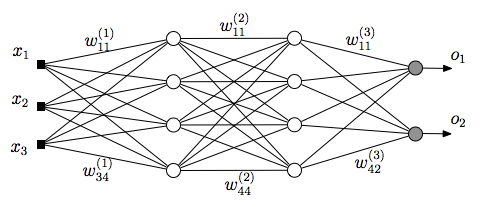
\includegraphics[scale=0.5]{img/MLP}
    \caption{Paveikslėlio pavyzdys}
    \label{img:mlp}
\end{figure}


\section{Eksperimentinio palyginimo rezultatai}
% tablesgenerator.com - converts calculators (e.g. excel) tables to LaTeX
\begin{table}[H]\footnotesize
  \centering
  \caption{Lentelės pavyzdys}
  {\begin{tabular}{|l|c|c|} \hline
    Algoritmas & $\bar{x}$ & $\sigma^{2}$ \\
    \hline
    Algoritmas A  & 1.6335    & 0.5584       \\
    Algoritmas B  & 1.7395    & 0.5647       \\
    \hline
  \end{tabular}}
  \label{tab:table example}
\end{table}

\end{document}
